\begin{solution}\\
Hay un total de $11$ teselaciones para $n=c$, es decir $c_5=11$. A continuación se muestran las teselaciones:
    \newcommand\drawRingB[3]{%
    % #1 es la lista separada por comas, p.e.: "90,180"
    % Agregamos comas delante y detrás:
    \edef\skipList{,#1,}%
    \begin{scope}[shift={(#2,#3)}]
      \draw[thick,fill=green!30] (0,0) circle (1);
      \draw[thick,fill=white] (0,0) circle (0.7);
    
      \foreach \a in {0,72,144,216,288} {
        \edef\angleAsText{,\a,}%
        \IfSubStr{\skipList}{\angleAsText}{%
           % \a está en la lista => omite dibujar
        }{%
           \draw[thick] (\a:0.7) -- (\a:1);
        }%
      }
    \end{scope}
    }
    \begin{center}
    \shorthandoff{>}
    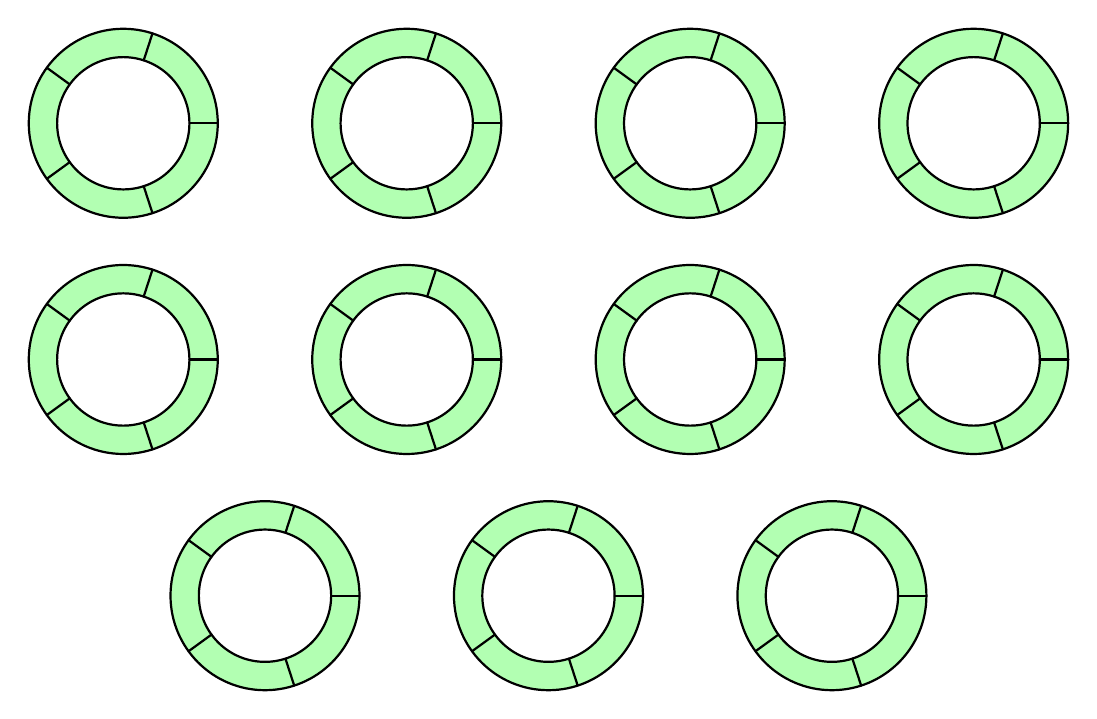
\begin{tikzpicture}[scale=1.2,cap=round,line join=round]
    % A helper macro to draw a "washer" (ring) of 5 arcs at position (#2,#3),
    % skipping radial boundaries whose angles are listed in #1.
    % #1 is a comma-separated list of angles, e.g. {72,216} means
    % "do *not* draw the boundary lines at 72° and 216°".
    %
    % For each ring:
    %   -- Outer radius = 1
    %   -- Inner radius = 0.7
    %
    
    % The 11 valid skip patterns for c5:
    %
    % Interpreting a 5-bit circular pattern:
    %  - '1' at position i => skip boundary at angle 72*i.
    %  - No two '1's are adjacent in a circular sense.
    % This yields exactly the following 11 sets:
    %
    % 1)  00000 -> skip none
    % 2)  10000 -> skip angle 0
    % 3)  01000 -> skip angle 72
    % 4)  00100 -> skip angle 144
    % 5)  00010 -> skip angle 216
    % 6)  00001 -> skip angle 288
    % 7)  10100 -> skip angles 0,144
    % 8)  01010 -> skip angles 72,216
    % 9)  00101 -> skip angles 144,288
    % 10) 10010 -> skip angles 0,216
    % 11) 01001 -> skip angles 72,288
    %
    % We will place them in a 4-column grid:
    % (Row 0)
    \drawRingB{}           {0}{0}      % no skips
    \drawRingB{0}          {3}{0}      % skip 0
    \drawRingB{72}         {6}{0}
    \drawRingB{144}        {9}{0}   
    % % (Row 1)
    \drawRingB{216}        {0}{-2.5}
    \drawRingB{288}        {3}{-2.5}
    \drawRingB{0,144}      {6}{-2.5}
    \drawRingB{0,216}      {9}{-2.5}
    % % (Row 2)
    \drawRingB{72,216}     {0+1.5}{-5}
    \drawRingB{72,288}     {3+1.5}{-5}
    \drawRingB{144,288}   {6+1.5}{-5}
    
    
    % % (Row 2)
    % \drawRing{144,288}    {0}{-6}
    % \drawRing{0,216}      {3}{-6}
    % \drawRing{72,288}     {6}{-6}
    \end{tikzpicture}
    \shorthandon{>}
    \end{center}
\end{solution}